% ---------------------------------------------------------------------
%  TFPT --- Safeguards against coincidence and numerology
%  The verification discipline: every mechanism by which TFPT defends a
%  load-bearing claim against chance, fitting and over-reading, expressed
%  uniformly (status calculus, no-free-pattern, over-determination map,
%  firewall, frozen predictions + null model, the independent Wolfram and
%  Lean paths, the red team, and the honest residual).
% ---------------------------------------------------------------------
\documentclass[11pt,a4paper]{article}
\usepackage[T1]{fontenc}
\usepackage[utf8]{inputenc}
\usepackage[english]{babel}
\usepackage{lmodern}
\usepackage[a4paper,margin=2.3cm]{geometry}
\usepackage{graphicx}
\usepackage{amsmath,amssymb,amsthm}
\usepackage{mathtools}
\usepackage{booktabs,array,tabularx}
\usepackage{enumitem}
\usepackage{xcolor}
\usepackage[most]{tcolorbox}
\usepackage{microtype}
\usepackage[hidelinks,colorlinks=true,linkcolor=blue!55!black,urlcolor=blue!55!black]{hyperref}
\emergencystretch=3em

% ---------------------------------------------------------------------
%  tfpt_style.tex -- THE shared visual style for every TFPT document.
%  Single source for colours, status markers, marker key, the \veri
%  script reference, the tcolorbox families, and the running
%  header/footer.  \input AFTER xcolor + tcolorbox[most] + hyperref are
%  loaded (every paper loads those).  Each document sets its short
%  running title before \begin{document}, e.g.
%        \def\TFPTdoctitle{Architecture and the E8 Compiler}
%  ---------------------------------------------------------------------
\usepackage{fancyhdr}
\usepackage{etoolbox}
\usepackage{tikz}
\usetikzlibrary{positioning,arrows.meta,fit,backgrounds,calc,shapes.geometric,shapes.misc}

% ---- single-source author / version / automatic date stamp ----
% ---------------------------------------------------------------------
%  tex-artefacts/version.tex -- single source for author list, version
%  and the automatic title-page date stamp of every TFPT document.
%  \input by tex-artefacts/tfpt_style.tex, so every paper that loads the
%  shared style automatically gets:
%     \TFPTauthors   -- the author list (use as \author{\TFPTauthors})
%     \TFPTversion   -- curated semantic version (bump per release; mirror
%                       the bump in changelog.tex)
%     \TFPTrev       -- auto build revision = git commit count, injected by
%                       build.sh into tex-artefacts/version-auto.tex
%                       (gitignored); falls back to "dev" for standalone runs
%     \TFPTdatestamp -- the title-page date line: \today + version + revision
%  build.sh also writes tex-artefacts/release-version.txt (gitignored):
%     "{TFPTversion} (rev {git commit count})" for Zenodo + release tooling.
%  Bump \TFPTversion here ONCE; it then updates in all papers at the next build.
% ---------------------------------------------------------------------
\def\TFPTauthors{Stefan Hamann \and Alessandro Rizzo}
\def\TFPTversion{5.3}
\def\TFPTrev{dev}
% build.sh regenerates the line below with the live git commit count:
\InputIfFileExists{tex-artefacts/version-auto.tex}{}{}
\def\TFPTdatestamp{\today\,\textperiodcentered\,v\TFPTversion\,(rev~\TFPTrev)}


% ---- colours (canonical TFPT palette) ----
\definecolor{tfblue}{HTML}{1F4E79}
\definecolor{tfgreen}{HTML}{1E7B45}
\definecolor{tfred}{HTML}{9B2226}
\definecolor{tfgold}{HTML}{B8860B}
\definecolor{tfgray}{HTML}{555555}

% ---- status markers (simplified 4-class display system) ----
% Reader-facing markers collapse to FOUR classes.  The fine-grained per-claim
% type (Axiom / Formal / Lattice / Numerical / Identity / Physical) stays in
% verification/status_ledger.csv -- the single source of truth -- so no fidelity
% is lost; the papers just show the coarse class so a reader is not overwhelmed.
%   [E] exact / machine-proven  (identity, Lie/lattice, formalised, numerical FP)
%   [C] conditional             (physical / bridge / readout, under named hypotheses)
%   [O] open / axiom            (declared input or genuine gap)
%   [X] kill test               (falsifiable threshold)
\newcommand{\mE}{{\small\textcolor{tfgreen!70!black}{\textbf{[E]}}}}
\newcommand{\mC}{{\small\textcolor{tfgold!78!black}{\textbf{[C]}}}}
\newcommand{\mO}{{\small\textcolor{tfred!80!black}{\textbf{[O]}}}}
\newcommand{\mX}{{\small\textcolor{tfred!58!black}{\textbf{[X]}}}}
% backward-compatible aliases: the old fine-grained names now render their class,
% so any not-yet-rewritten call site (or the standalone changelog) still compiles.
\newcommand{\tI}{\mE}\newcommand{\tL}{\mE}\newcommand{\tF}{\mE}\newcommand{\tN}{\mE}
\newcommand{\tIalg}{\mE}\newcommand{\tInum}{\mE}
\newcommand{\tP}{\mC}\newcommand{\tB}{\mC}\newcommand{\tR}{\mC}
\newcommand{\tA}{\mO}
\newcommand{\tX}{\mX}

% compact marker legend, placed under a marker-bearing table
\newcommand{\markerkey}{\par\vspace{1.5pt}\noindent{\scriptsize\itshape
  \textcolor{black!58}{Marker key:\ \mE~exact / machine-proven\,$\cdot$\,%
  \mC~conditional (holds under named hypotheses)\,$\cdot$\,%
  \mO~open / axiom\,$\cdot$\,\mX~falsifiable kill test.\ \
  Per-claim fine type in \texttt{verification/status\_ledger.csv}.}}\par\vspace{2pt}}

% horizontal badge bar (place once near the front of a document)
\newcommand{\TFPTbadges}{\par\noindent
  \fcolorbox{tfgreen!55!black}{tfgreen!8}{\scriptsize\mE\,exact / machine-proven}\hfill
  \fcolorbox{tfgold!70!black}{tfgold!10}{\scriptsize\mC\,conditional}\hfill
  \fcolorbox{tfred!75!black}{tfred!8}{\scriptsize\mO\,open / axiom}\hfill
  \fcolorbox{tfred!60!black}{tfred!6}{\scriptsize\mX\,kill test}\par\vspace{3pt}}

% inline reference to the script that machine-checks a claim (see verification/)
\newcommand{\veri}[1]{\,{\footnotesize\textcolor{tfblue!70!black}{[\,\texttt{verification/#1}\,]}}}
% lightweight inline colour-mark for a bare verification-script token in running
% prose / tables, e.g. \vref{v108}, \vref{v49}/\vref{v71}.  Same blue as \veri so a
% reader instantly sees "this is a machine-checked module reference".
\newcommand{\vref}[1]{\textcolor{tfblue!72!black}{\textsf{#1}}}

% ---- tcolorbox families (one visual language across all documents) ----
% keybox  : the central claim / reading of a section (blue)
% winbox  : an established result / closure (green)
% gapbox  : an open gate / honest caveat / kill criterion (red)
% auditbox: a recorded audit fingerprint, not load-bearing (gold)
% navbox  : a light, neutral navigation / reference card (document map, etc.)
% Visual language (deliberately light): a faint tint, a thin coloured frame
% and a light title band with dark coloured title text -- NOT a heavy
% white-on-saturated-colour bar -- so a page never reads as a wall of boxes.
\newtcolorbox{keybox}[1][]{enhanced,breakable,boxrule=0.5pt,arc=1.5pt,
  colback=tfblue!4!white,colframe=tfblue!70!black,coltitle=tfblue!88!black,colbacktitle=tfblue!12!white,
  fonttitle=\bfseries\small,fontupper=\small,title={#1},left=2mm,right=2mm,top=1mm,bottom=1mm}
% non-breaking variant (front-matter cards that should never split across a page)
\newtcolorbox{keyboxnb}[1][]{enhanced,breakable=false,boxrule=0.5pt,arc=1.5pt,
  colback=tfblue!4!white,colframe=tfblue!70!black,coltitle=tfblue!88!black,colbacktitle=tfblue!12!white,
  fonttitle=\bfseries\small,fontupper=\small,title={#1},left=2mm,right=2mm,top=1mm,bottom=1mm}
\newtcolorbox{winbox}[1][]{enhanced,breakable,boxrule=0.5pt,arc=1.5pt,
  colback=tfgreen!5!white,colframe=tfgreen!65!black,coltitle=tfgreen!50!black,colbacktitle=tfgreen!14!white,
  fonttitle=\bfseries\small,fontupper=\small,title={#1},left=2mm,right=2mm,top=1mm,bottom=1mm}
\newtcolorbox{gapbox}[1][]{enhanced,breakable,boxrule=0.5pt,arc=1.5pt,
  colback=tfred!4!white,colframe=tfred!70!black,coltitle=tfred!75!black,colbacktitle=tfred!12!white,
  fonttitle=\bfseries\small,fontupper=\small,title={#1},left=2mm,right=2mm,top=1mm,bottom=1mm}
% non-breaking variants (callouts that must stay whole on one page, embedded in text)
\newtcolorbox{winboxnb}[1][]{enhanced,breakable=false,boxrule=0.5pt,arc=1.5pt,
  colback=tfgreen!5!white,colframe=tfgreen!65!black,coltitle=tfgreen!50!black,colbacktitle=tfgreen!14!white,
  fonttitle=\bfseries\small,fontupper=\small,title={#1},left=2mm,right=2mm,top=1mm,bottom=1mm}
\newtcolorbox{gapboxnb}[1][]{enhanced,breakable=false,boxrule=0.5pt,arc=1.5pt,
  colback=tfred!4!white,colframe=tfred!70!black,coltitle=tfred!75!black,colbacktitle=tfred!12!white,
  fonttitle=\bfseries\small,fontupper=\small,title={#1},left=2mm,right=2mm,top=1mm,bottom=1mm}
\newtcolorbox{auditbox}[1][]{enhanced,breakable,boxrule=0.5pt,arc=1.5pt,
  colback=tfgold!7!white,colframe=tfgold!70!black,coltitle=tfgold!45!black,colbacktitle=tfgold!16!white,
  fonttitle=\bfseries\small,fontupper=\small,title={#1},left=2mm,right=2mm,top=1mm,bottom=1mm}
\newtcolorbox{navbox}[1][]{enhanced,breakable,boxrule=0.5pt,arc=1.5pt,
  colback=tfgray!3!white,colframe=tfgray!55,coltitle=tfgray!30!black,colbacktitle=tfgray!12!white,
  fonttitle=\bfseries\small,fontupper=\small,title={#1},left=2mm,right=2mm,top=1mm,bottom=1mm}
% back-compatibility aliases (older box names map onto the canonical types)
\newtcolorbox{audbox}[1][]{enhanced,breakable,boxrule=0.5pt,arc=1.5pt,
  colback=tfgold!7!white,colframe=tfgold!70!black,coltitle=tfgold!45!black,colbacktitle=tfgold!16!white,
  fonttitle=\bfseries\small,fontupper=\small,title={#1},left=2mm,right=2mm,top=1mm,bottom=1mm}
\newtcolorbox{resbox}[1][]{enhanced,breakable,boxrule=0.5pt,arc=1.5pt,
  colback=tfgreen!5!white,colframe=tfgreen!55!black,coltitle=tfgreen!50!black,colbacktitle=tfgreen!12!white,
  fonttitle=\bfseries\small,fontupper=\small,title={#1},left=2mm,right=2mm,top=1mm,bottom=1mm}
\newtcolorbox{roadbox}[1][]{enhanced,breakable,boxrule=0.5pt,arc=1.5pt,
  colback=tfgreen!5!white,colframe=tfgreen!55!black,coltitle=tfgreen!50!black,colbacktitle=tfgreen!12!white,
  fonttitle=\bfseries\small,fontupper=\small,title={#1},left=2mm,right=2mm,top=1mm,bottom=1mm}
\newtcolorbox{intbox}[1][]{enhanced,breakable,boxrule=0.5pt,arc=1.5pt,
  colback=tfgold!7!white,colframe=tfgold!70!black,coltitle=tfgold!45!black,colbacktitle=tfgold!16!white,
  fonttitle=\bfseries\small,fontupper=\small,title={#1},left=2mm,right=2mm,top=1mm,bottom=1mm}

% ---- colour-marked display formula (load-bearing key equations) ----
% A highlighted formula line: a coloured left accent bar + faint tint, no full
% frame -- so a key equation is visually set apart from the running prose
% without becoming yet another box.  Use:  \begin{keyeq}$\displaystyle ...$\end{keyeq}
\newtcolorbox{keyeq}{blanker,breakable=false,halign=center,
  colback=tfgold!8!white,borderline west={2.4pt}{0pt}{tfgold!75!black},
  left=8pt,right=6pt,top=3pt,bottom=3pt,before skip=5pt,after skip=5pt}

% ---- running header / footer (consistent across all documents) ----
\providecommand{\TFPTdoctitle}{}
\setlength{\headheight}{14pt}
\pagestyle{fancy}
\fancyhf{}
\fancyhead[L]{\footnotesize\textcolor{tfgray}{\textit{TFPT}\,\textbullet\,\TFPTdoctitle}}
\fancyhead[R]{\footnotesize\textcolor{tfgray}{\thepage}}
\fancyfoot[L]{\scriptsize\textcolor{tfgray}{v\TFPTversion\,\textperiodcentered\,rev~\TFPTrev}}
\renewcommand{\headrulewidth}{0.3pt}
\renewcommand{\footrulewidth}{0pt}
\fancypagestyle{plain}{\fancyhf{}\renewcommand{\headrulewidth}{0pt}%
  \fancyfoot[C]{\footnotesize\textcolor{tfgray}{\thepage}}%
  \fancyfoot[L]{\scriptsize\textcolor{tfgray}{v\TFPTversion\,\textperiodcentered\,rev~\TFPTrev}}}

% ---- shared figure macros (claim stack, anchor cockpit, E8 glue, 2/3 motif, K5) ----
%  (this fragment lives in tex-artefacts/ and is \input by documents compiled from
%   the repository root, so the path is given relative to that root.)
% ---------------------------------------------------------------------
%  tfpt_figures.tex -- shared, reusable TikZ figure macros for every
%  TFPT document.  \input by tfpt_style.tex (which loads tikz + the
%  needed libraries + etoolbox).  Each macro draws a self-contained
%  centred figure; nothing is drawn until the macro is called.
%
%    \TFPTclaimstack[zone]  -- the architecture claim stack (B3); the
%                              optional zone in {axioms,anchor,compiler,
%                              sm,bridges,frontier} is highlighted.
%    \TFPTanchorcockpit      -- the anchor a=(1,1,2) cockpit (B4)
%    \TFPTeightglue          -- the D5 (+) A3 +mu4 => E8 glue (B5)
%    \TFPTmotif              -- the 2/3 motif map (B6)
%    \TFPTactionkfive        -- the K5 action-lattice mnemonic (B7)
% ---------------------------------------------------------------------

% ===== B3: the architecture claim stack =========================
\newcommand{\tfhl}[1]{\ifdefstring{\tfcur}{#1}{cbhi}{cbnl}}
\newcommand{\TFPTclaimstack}[1][none]{%
\def\tfcur{#1}%
\begin{center}
\begin{tikzpicture}[font=\footnotesize,
  cb/.style={rounded corners=2pt,inner sep=4pt,text width=118mm,align=center,minimum height=8.5mm},
  cbnl/.style={line width=0.5pt}, cbhi/.style={line width=1.5pt},
  ar/.style={-{Stealth[length=2.2mm]},tfgray,semithick}]
  \node[cb,fill=tfred!8,draw=tfred!75!black,\tfhl{axioms}] (axioms)
    {\textbf{P1}\,$c_3=\tfrac1{8\pi}$ \quad \textbf{P2}\,$g_{\mathrm{car}}=5$ \ \textcolor{tfgray}{\itshape(two inputs, [O] axioms)}};
  \node[cb,fill=tfblue!8,draw=tfblue,\tfhl{anchor},below=3.5mm of axioms] (anchor)
    {Anchor $a=(1,1,2)$:\ $e_1,e_2,e_3=4,5,2$ \ \textcolor{tfgray}{\itshape([E] exact)}};
  \node[cb,fill=tfgreen!10,draw=tfgreen!70!black,\tfhl{compiler},below=3.5mm of anchor] (compiler)
    {Discrete compiler:\ $D_5\oplus A_3+\mu_4\Rightarrow E_8$,\ $h=30$,\ $\varphi_0$ \ \textcolor{tfgray}{\itshape([E] exact)}};
  \node[cb,fill=tfgreen!7,draw=tfgreen!60!black,\tfhl{sm},below=3.5mm of compiler] (sm)
    {SM skeleton:\ three families, hypercharges, flavor matrix $R$ \ \textcolor{tfgray}{\itshape([E])}};
  \node[cb,fill=tfgold!12,draw=tfgold!80!black,\tfhl{bridges},below=3.5mm of sm] (bridges)
    {Physical bridges:\ $v_{\mathrm{geo}}$,\ $G_{\mathrm{net}}$,\ $F_{\mathrm{transfer}}$ \ \textcolor{tfgray}{\itshape([C] bridges)}};
  \node[cb,fill=tfgray!12,draw=tfgray!70!black,\tfhl{frontier},below=3.5mm of bridges] (frontier)
    {Frontier readouts:\ $\Lambda$, inflation, $\eta_B$, dark matter, QG \ \textcolor{tfgray}{\itshape([C]/[O])}};
  \draw[ar] (axioms)--(anchor); \draw[ar] (anchor)--(compiler);
  \draw[ar] (compiler)--(sm);   \draw[ar] (sm)--(bridges); \draw[ar] (bridges)--(frontier);
\end{tikzpicture}
\end{center}}

% ===== B4: the anchor cockpit ====================================
\newcommand{\TFPTanchorcockpit}{%
\begin{center}
\begin{tikzpicture}[font=\footnotesize,
  pan/.style={rounded corners=2pt,draw=tfblue!60,fill=tfblue!4,inner sep=5pt,
    text width=46mm,align=left},
  hd/.style={font=\bfseries\small,tfblue}]
  \node[pan] (e) {\textbf{elementary} $e_k(a)$\\[2pt]
     $e_1=4\to|\mu_4|$\\ $e_2=5\to g_{\mathrm{car}}$\\ $e_3=2\to|\mathbb Z_2|$\\[2pt]
     $c_3=\tfrac1{2e_1\pi}=\tfrac1{8\pi}$};
  \node[pan,right=4mm of e] (p) {\textbf{power sums} $p_n=2+2^n$\\[2pt]
     $p_0,p_1,p_2,p_3=3,4,6,10$\\ $p_1p_2p_3=240=|R(E_8)|$\\ $p_4-p_3=8=\operatorname{rank}E_8$\\
     $\Rightarrow\dim E_8=248$};
  \node[pan,right=4mm of p] (m) {\textbf{derived motifs}\\[2pt]
     $4,5,8,16,25,$\\ $30,41,120,240$\\[2pt]
     \textcolor{tfgray}{\itshape one anchor,}\\ \textcolor{tfgray}{\itshape many projections}};
  \node[hd,above=1mm of p.north] {$a=(1,1,2)$ \ \textcolor{tfgray}{\footnotesize\itshape[E]}};
\end{tikzpicture}
\end{center}}

% ===== B5: the E8 glue ===========================================
\newcommand{\TFPTeightglue}{%
\begin{center}
\begin{tikzpicture}[font=\footnotesize,
  d/.style={rounded corners=2pt,draw=tfblue,fill=tfblue!6,inner sep=4pt,align=center,text width=36mm},
  mid/.style={rounded corners=2pt,draw=tfgold!80!black,fill=tfgold!12,inner sep=4pt,align=center,text width=52mm},
  e8/.style={rounded corners=2pt,draw=tfgreen!70!black,fill=tfgreen!10,inner sep=4pt,align=center,text width=52mm,font=\bfseries},
  rt/.style={rounded corners=2pt,draw=tfgreen!55!black,fill=tfgreen!6,inner sep=3pt,align=center,text width=52mm},
  side/.style={rounded corners=2pt,draw=tfgray!55,fill=tfgray!6,inner sep=4pt,align=left,text width=34mm,font=\scriptsize},
  ar/.style={-{Stealth[length=2mm]},tfgray,semithick}]
  \node[d] (d5) {$D_5$ discriminant\\ $\mathbb Z_4$, $q=5/4$};
  \node[d,right=10mm of d5] (a3) {$A_3$ discriminant\\ $\mathbb Z_4$, $q=3/4$};
  \node[mid,below=5mm of $(d5)!0.5!(a3)$] (glue) {$\mu_4$ anti-isometry\ ($q$-sum $=2$)};
  \node[e8,below=4mm of glue] (e8) {even unimodular $E_8$ lattice};
  \node[rt,below=4mm of e8] (rt) {$240$ roots,\ rank $8$,\ $\dim=248$};
  \node[side,right=8mm of glue] (why) {\textbf{why unique?}\\ rank $8$\\ even\\ unimodular\\ positive definite};
  \draw[ar] (d5)--(glue); \draw[ar] (a3)--(glue);
  \draw[ar] (glue)--(e8); \draw[ar] (e8)--(rt);
\end{tikzpicture}\\[2pt]
{\scriptsize\itshape $D_5\oplus A_3+\mu_4\Rightarrow E_8$ --- the unique even unimodular rank-$8$ glue \ [E] exact (lattice).}
\end{center}}

% ===== B5b: the double pushout (one glue, two categories) ========
\newcommand{\TFPTdoublepushout}{%
\begin{center}
\begin{tikzpicture}[font=\footnotesize,>={Stealth[length=2mm]},
  lat/.style={rounded corners=2pt,draw=tfblue,fill=tfblue!6,inner sep=5pt,align=center,text width=34mm},
  net/.style={rounded corners=2pt,draw=tfblue!70!black,fill=tfblue!4,inner sep=5pt,align=center,text width=34mm},
  e8l/.style={rounded corners=2pt,draw=tfgold!80!black,fill=tfgold!12,inner sep=5pt,align=center,text width=34mm,font=\bfseries},
  e8n/.style={rounded corners=2pt,draw=tfgreen!70!black,fill=tfgreen!10,inner sep=5pt,align=center,text width=34mm,font=\bfseries},
  ar/.style={->,tfgray,semithick},
  lb/.style={font=\scriptsize,text=black,align=center,fill=white,inner sep=1.5pt}]
  \node[lat] (LL) at (0,2.5)   {$D_5\oplus A_3$\\[1pt]\scriptsize root lattices,\ $\mathrm{disc}=\Z_4$};
  \node[e8l] (LR) at (6.6,2.5) {$E_8$\\[1pt]\scriptsize even unimodular,\ $\det 1$};
  \node[net] (BL) at (0,0)     {$(D_5)_1\otimes(A_3)_1$\\[1pt]\scriptsize chiral nets,\ $c=8$};
  \node[e8n] (BR) at (6.6,0)   {$(E_8)_1$\\[1pt]\scriptsize holomorphic,\ $\mu$-index $1$};
  \draw[ar] (LL)--node[lb]{$+\,\mu_4$ glue}(LR);
  \draw[ar] (BL)--node[lb]{$\rtimes\,\mu_4$ extension}(BR);
  \draw[ar] (LL)--node[lb,left=-1pt]{level-$1$}(BL);
  \draw[ar] (LR)--node[lb,right=-1pt]{level-$1$}(BR);
\end{tikzpicture}\\[2pt]
{\scriptsize\itshape One operation, two categories: the order-$|\mu_4|{=}4$ glue is the lattice pushout
$D_5\oplus A_3+\mu_4\Rightarrow E_8$ \emph{and} the simple-current / anyon-condensation extension
$(D_5)_1\otimes(A_3)_1\rtimes\mu_4\cong(E_8)_1$; the square commutes. \ [E] exact.}
\end{center}}

% ===== B6: the 2/3 motif map =====================================
\newcommand{\TFPTmotif}{%
\begin{center}
\begin{tikzpicture}[font=\footnotesize,
  ex/.style={rounded corners=2pt,draw=tfgreen!70!black,fill=tfgreen!8,inner sep=4pt,align=center,text width=92mm},
  br/.style={rounded corners=2pt,draw=tfgold!80!black,fill=tfgold!12,inner sep=4pt,align=center,text width=92mm},
  ar/.style={-{Stealth[length=2mm]},tfgray,semithick}]
  \node[ex] (a) {$|\mathbb Z_2|/N_{\mathrm{fam}}=2/3$ \ \textcolor{tfgray}{\itshape(anchor ratio)}};
  \node[ex,below=3mm of a] (b) {parabolic weights $\{0,\tfrac13,\tfrac23\}=\operatorname{spec}A_0^\star$};
  \node[ex,below=3mm of b] (c) {transfer spectrum $\{1,(2/3)^6,(1/3)^6\}$,\ gap $6\log\tfrac32$};
  \node[br,below=3mm of c] (d) {Koide target $2/3$ \ \textcolor{tfgray}{\itshape(source$\to$pole bridge [C])}};
  \node[br,below=3mm of d] (e) {Nariai / horizon entropy bound $2/3$ \ \textcolor{tfgray}{\itshape([C])}};
  \draw[ar] (a)--(b); \draw[ar] (b)--(c); \draw[ar] (c)--(d); \draw[ar] (d)--(e);
\end{tikzpicture}\\[2pt]
{\scriptsize\itshape Green: exact motif ([E]).\quad Gold: physical bridge ([C]) --- the same ratio, two epistemic types.}
\end{center}}

% ===== B7: the K5 action-lattice mnemonic ========================
%  Layout: complete graph K5 (pentagon, all 10 edges) on the LEFT, the
%  Pascal-row reading list on the RIGHT, vertically centred on the graph
%  so the two blocks never overlap.
\newcommand{\TFPTactionkfive}{%
\begin{center}
\begin{tikzpicture}[font=\scriptsize]
  % --- K5 vertices on a regular pentagon, centred at the origin ---
  \foreach \i in {1,...,5}{\coordinate (k\i) at ({90+72*(\i-1)}:12mm);}
  \begin{scope}[on background layer]
    \foreach \i in {1,...,5}{\foreach \j in {1,...,5}{\ifnum\i<\j
      \draw[tfgray!55,line width=0.5pt] (k\i)--(k\j);\fi}}
  \end{scope}
  \foreach \i in {1,...,5}{\fill[tfblue!70!black] (k\i) circle (1.8pt);}
  \node[tfgray,font=\scriptsize\itshape] at (0,-1.9) {$K_5$};
  % --- reading list, anchored to the right of the whole graph, centred ---
  \node[anchor=west,align=left,inner sep=0pt] at (1.9cm,0) {%
    $\tbinom51=5$\ \ vertices --- action $x^1$ (Hubble slot)\\[1pt]
    $\tbinom52=10$\ edges --- $\Lambda$ density pair $x^{10}$\\[1pt]
    $\tbinom53=10$\ triangles --- dual sector\\[1pt]
    $\tbinom54=5$\ \ complements --- inverse sector\\[1pt]
    $\tbinom55=1$\ \ determinant --- closure};
\end{tikzpicture}\\[2pt]
{\scriptsize\itshape $K_5$ on the five carrier slots; the action powers $x^{1},x^{5},x^{10}$ are its
$\tbinom5k$ faces \ \textcolor{tfgray}{(mnemonic; the physical scale map stays [C]).}}
\end{center}}


\newcommand{\phiz}{\varphi_0^{\mathrm{ret}}}
\newcommand{\cthree}{c_3}
\newcommand{\Mpl}{\bar M_{\mathrm{Pl}}}
\newcommand{\Nfam}{N_{\mathrm{fam}}}
\newcommand{\gcar}{g_{\mathrm{car}}}
\newcommand{\ainv}{\alpha^{-1}}
\newcommand{\PP}{\mathbb P^1}
\newcommand{\Z}{\mathbb Z}
\setlist{itemsep=2pt,topsep=3pt}
\newcolumntype{Y}{>{\raggedright\arraybackslash}X}

\title{\vspace{-1.2cm}\textbf{TFPT --- Safeguards against Coincidence and Numerology}\\[2mm]
\large The verification discipline: how every load-bearing claim is defended against chance,
fitting and over-reading}
\author{\TFPTauthors}\date{\TFPTdatestamp}

\def\TFPTdoctitle{Safeguards}
\begin{document}
\maketitle

% ---------------------------------------------------------------------
%  tfpt_docset.tex -- THE canonical TFPT document-set box.
%  Single source of truth for the document list; \input by the
%  introduction and every paper. Uses only universally available
%  macros (keybox + plain LaTeX math) so it compiles in every doc.
%  Each document adds its own "You are reading ..." line directly
%  after the \input.  Numbering is aligned with the file names:
%  document N == tfpt_N_*, the introduction is the entry point, and
%  R/H/O are the appendix-style companions.
% ---------------------------------------------------------------------
\begin{navbox}[The TFPT document set --- what is treated where]
\textbf{Plain language:} TFPT (Topological Fixed-Point Theory) is a small discrete compiler. Two
inputs --- the seam constant $c_3=\tfrac1{8\pi}$ and the carrier rank $g_{\mathrm{car}}=5$ --- build
$D_5\oplus A_3+\mu_4\Rightarrow E_8$ and read off the Standard-Model skeleton, the constants and the
scale grammar. The series is \textbf{the introduction plus five numbered papers and three companions},
best read in order:
\begin{enumerate}[leftmargin=2.0em,itemsep=1pt,label=\textbf{\arabic*.}]
\setcounter{enumi}{-1}
\item \texttt{introduction} --- reading guide, compiler closure, predictions, the dependency DAG and the
      single proof ledger (\texttt{verification/status\_ledger.csv}). \emph{(entry point)}
\item \texttt{tfpt\_1\_architecture\_e8} --- the two axioms, the derivation map, the EM fixed point
      $\alpha^{-1}$, the $D_5\oplus A_3+\mu_4\Rightarrow E_8$ construction, the QBL theorem chain.
\item \texttt{tfpt\_2\_standard\_model} --- the SM in one $\varphi_0$-ladder formula, flavor from
      parabolic transport (sheet diamond, dual anchor, $Q_+$ cohomology), the worked closures.
\item \texttt{tfpt\_3\_e8\_audit\_bootstrap} --- the seven $E_8$ slices as an audit raster, the cascade
      bridge, the M\"obius bootstrap.
\item \texttt{tfpt\_4\_frontier} --- honest status of $\eta_B$, $m_p/m_e$, Koide, dark matter, full QG.
\item \texttt{tfpt\_5\_redteam} --- the adversarial audit: declared attacks, what survives, what each
      reduces to, and the kill tests.
\end{enumerate}
\noindent\textbf{Companions:} \textbf{R.} \texttt{tfpt\_research\_contracts} --- the open interfaces
$(v_{\mathrm{geo}}, G_{\mathrm{net}}, F_{\mathrm{transfer}})$ as numbered contracts;
\textbf{H.} \texttt{tfpt\_horizon\_readouts} --- Appendix~H (unit-system reframe): one seam constant as
the universal horizon thermal code, the Nariai/anchor surface, the resummed seam clock;
\textbf{O.} \texttt{origin\_theory} --- why no free fundamental number remains (exact core $+$ one
honestly-typed cyclic interpretation).
\end{navbox}

\noindent\emph{You are reading the \textbf{Safeguards} companion (S): it collects, in one place and in
one language, every mechanism by which TFPT protects a claim against coincidence --- the status
calculus, the anti-fitting rules, the over-determination accounting, the firewall, the frozen
predictions and null model, the two independent proof paths (Wolfram, Lean), the red team, and the
honest residual. It introduces no new physics; it makes the discipline auditable.}

\begin{abstract}
\noindent A two-input theory that reads out many small integers is, a priori, at risk of being
elaborate numerology. TFPT answers that risk not with rhetoric but with a \emph{layered, machine-checked
discipline}, and this companion states all of it uniformly. The layers are: (1) a four-class status
calculus with a single-source ledger and a sync audit that forbids a conditional claim from being
rendered as exact; (2) an anti-fitting rule (``no free pattern'') plus a reverse audit that counts how
much structure carries \emph{no} readout; (3) an over-determination map that honestly separates
\emph{multiplicative} evidence from \emph{compression} (many readouts from one generator) and, applied to
TFPT's own arithmetic witnesses, finds them to be facets of \emph{one} $(2,3,5)/E_8$ object (compression),
locating the genuine multiplication in an input forced four independent ways plus a foreign readout
($\alpha^{-1}$); (4) a firewall that keeps external-physics interfaces from ever
being typed as compiler outputs, together with the No-Unit theorem that makes the absence of an absolute
scale a \emph{theorem}; (5) a frozen prediction registry with a Monte-Carlo null model and a live data
scorecard; (6) two independent reproduction paths --- an independent Wolfram engine and a Lean~4 kernel
proof; (7) an adversarial red-team layer; and a final, explicit statement of what would still falsify the
theory. The thesis is deliberately modest: these safeguards make coincidence an \emph{expensive}
explanation of the discrete core, and they keep ``exact compiler closure'' from ever being mistaken for
``closed physics''.
\end{abstract}

\section{The risk, and the shape of the answer}
The honest danger for TFPT is not that an individual number is wrong --- the arithmetic is usually clean
--- but \emph{closure inflation}: that an exact, discrete \emph{compiler} closure is read, or worded, as a
\emph{physical} closure. Every safeguard below exists to hold that one line. None of them, alone, turns
syntax into semantics; together they make the discrete core hard to dismiss as chance and impossible to
oversell as a finished Theory of Everything. We state each as a \emph{layer} with its enforcing
artefact(s).
\begin{figure}[ht]\centering
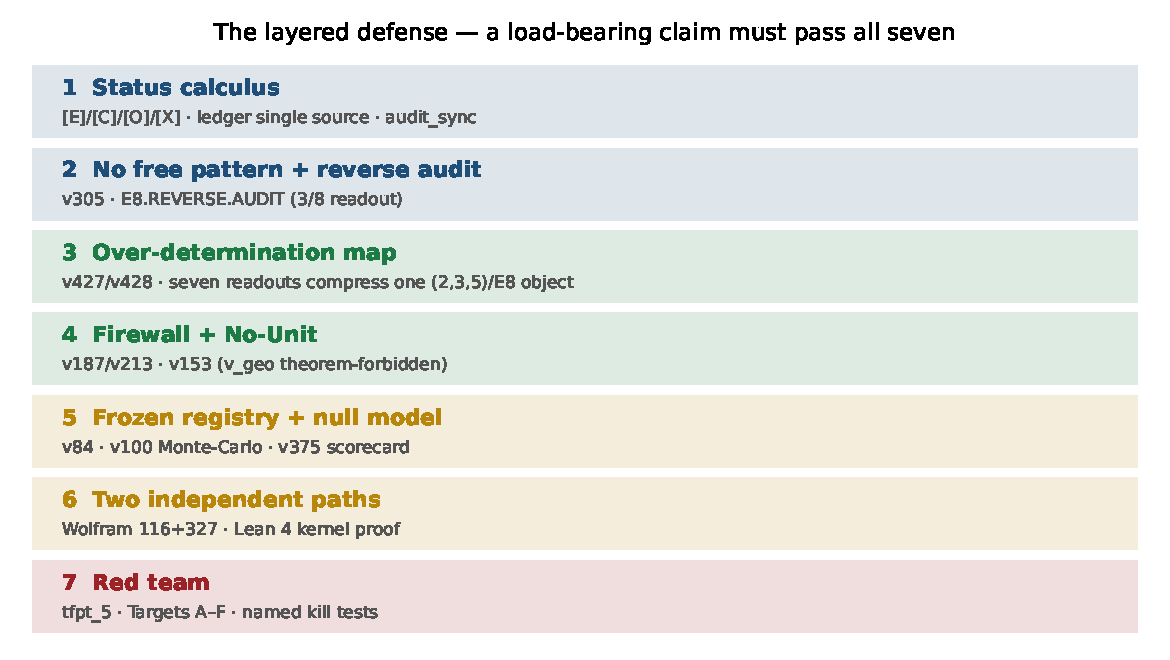
\includegraphics[width=0.86\linewidth]{figures/safeguard_layers}
\caption{The seven safeguard layers; a load-bearing claim must pass all of them. Each layer names its
enforcing artefact (script id or document).}\label{fig:layers}
\end{figure}

\section{Layer 1 --- the status calculus (no \texttt{[C]} dressed as \texttt{[E]})}
Every claim carries one of four display markers: \mE\ exact / proven (identity, Lie/lattice theorem,
Lean-formalised, or numerical fixed point), \mC\ conditional (physical, under named hypotheses), \mO\ open
/ axiom / anchor, \mX\ falsifiable kill test. The finer per-claim type (Axiom / Formal / Lattice /
Numerical / Identity / Physical) lives in the \emph{single source of truth},
\texttt{verification/status\_ledger.csv}; the papers and the website only \emph{mirror} it. A sync audit
(\texttt{verification/audit\_sync.py}, run as \texttt{bash build.sh audit}) enforces, in both directions,
that the suite, the runner, the registry and the ledger agree; that every script is cited in a paper
\emph{body}; and that no generated surface is stale. The point of the calculus is exactly the reviewer's
concern: it is structurally impossible for a \mC\ claim to be silently rendered as \mE, because the marker
is read from the ledger, not retyped per document.

\section{Layer 2 --- no free pattern, and the reverse audit}
\begin{keybox}[Anti-fitting: an identity earns its keep or it is decorative]
The \emph{forward discipline} / generator-economy audit (\veri{v305\_witness\_independence.py}, null model
\veri{v100\_numerology\_null\_mc.py}) admits an identity as load-bearing only if it is derivationally
necessary, kills alternatives, is ablation-relevant, links modules, or is experimentally testable;
admissible invariant classes are bounded in advance. The complementary \emph{reverse audit}
(\texttt{E8.REVERSE.AUDIT.01}) asks the honest
opposite question --- how much $E_8$ structure maps onto \emph{nothing}? Of the eight Casimir degrees
$\{2,8,12,14,18,20,24,30\}$, exactly \textbf{three} feed a primary physical readout (degree $2$, the
metric; degree $8$, the rank $\to\cthree=1/(8\pi)$; degree $30$, the Coxeter number $\to\gcar=5$ and the
order-$30$ clock) and \textbf{five} carry no primary readout. A theory that publishes its $5/8$ unused
overhead is not cherry-picking.
\end{keybox}
\begin{figure}[ht]\centering
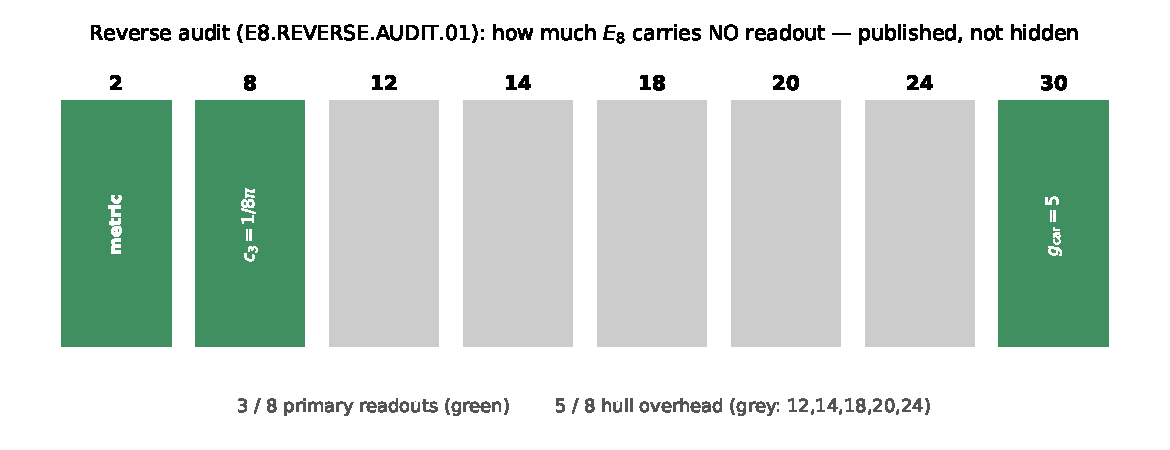
\includegraphics[width=0.84\linewidth]{figures/safeguard_reverse_audit}
\caption{The reverse audit (\texttt{E8.REVERSE.AUDIT.01}): of $E_8$'s eight Casimir degrees only three feed
a primary readout; the other five are published hull overhead.}\label{fig:reverse}
\end{figure}

\section{Layer 3 --- the over-determination map (multiply vs.\ compress)}
The strongest positive evidence is over-determination, but it must be counted honestly. The
\emph{framework} is a sharp axis (\veri{v427\_overdet\_witness\_map.py}, extending the generator-economy
audit \vref{v305}): evidence \emph{multiplies} only across genuinely disjoint grammars; many readouts
from one generator are a \emph{compression} gain, not independent multiplication. The hard part is
classifying TFPT's own witnesses correctly --- and applying that test to ourselves
(\veri{v428\_overdet\_reclass.py}) forces a self-correction that we state in full.
\begin{keybox}[Seven arithmetic readouts --- and why they \emph{compress}]
Each integer below is computed \emph{from its own grammar} and lands on a carrier-skeleton value:
\[
\begin{array}{lll}
\text{Gauss } \Z[i]: & N(3{+}2i)=3^2{+}2^2 & = 13\;(=\Delta_Q)\\
\text{Eisenstein } \Z[\omega]: & N(3{+}2\omega)=3^2{-}3\!\cdot\!2{+}2^2 & = 7\\
\text{Cyclotomy } \mathbb Q(\zeta_5): & N(3{+}2\zeta_5)=2^4\,\Phi_5(-3/2) & = 55\\
\text{Galois } (\Z/5)^\times: & |\!\operatorname{Gal}\mathbb Q(\zeta_5)|=\varphi(5) & = 4\;(=|\mu_4|)\\
\text{Root lattice}: & |\!\det\mathrm{Cartan}(E_8)| & = 1\\
\text{Pascal/exterior}: & \tbinom40{+}\tbinom41{+}\tbinom42 = 11,\;\; 2^4 & = 16=\dim S^+\\
\text{Coxeter}: & h(E_8)=30=2\!\cdot\!3\!\cdot\!5,\;\; \varphi(30) & = 8=\operatorname{rank}E_8
\end{array}
\]
These are seven \emph{syntactically} distinct grammars --- but syntactic distinctness is not statistical
independence. By the Brieskorn classification (\vref{v236}) the $(2,3,5)$ singularity $x^2{+}y^3{+}z^5$ is
the \emph{one} generator behind the order-$30$ clock, with Milnor number $\mu=(2{-}1)(3{-}1)(5{-}1)=8=
\operatorname{rank}E_8$ and $30=2\!\cdot\!3\!\cdot\!5=h(E_8)$. Each readout above is a facet of that same
object: $\Z[i]$ is the prime-$2$ ($\mu_4$/sheet) face, $\Z[\omega]$ the prime-$3$ (family) face,
$\mathbb Q(\zeta_5)$ and the Galois group the prime-$5$ (carrier) face, Pascal the $\mu_4$ exterior, the
Coxeter number the whole clock, and $\det\mathrm{Cartan}(E_8)$ the $E_8$ resolution itself. \emph{So the
seven do not multiply --- they compress}, exactly like the anchor $a=(1,1,2)$ emitting
$(e_1,e_2,e_3)=(4,5,2)$, the power sums, and the $E_8$ data from one generator. An earlier version of this
section called the seven ``disjoint grammars that multiply''; \veri{v428\_overdet\_reclass.py} applies
this layer's own test to that claim and walks it back.
\end{keybox}
\begin{keybox}[What honestly multiplies: forced inputs $+$ a foreign witness]
The genuine over-determination is of a different shape. First, the \emph{input} of the theory is forced
by several \emph{independent} arguments: the ``$8$'' in $c_3=1/(8\pi)$ equals $\operatorname{rank}E_8=8$,
the carrier Coxeter number $h(D_5)=2(5{-}1)=8$, the totient $\varphi(30)=8$, and the Milnor number
$(2{-}1)(3{-}1)(5{-}1)=8$ --- four \emph{different} mathematical facts that independently fix the same
constant, and that genuinely multiply. Second, the constant the theory was \emph{not} built around ---
$\alpha^{-1}\approx 137$, a prime foreign to the $(2,3,5)$ skeleton --- is reproduced as the fixed point
of the boundary Ward identity (\vref{v305}). The honest claim is therefore narrower and harder to attack:
not ``seven independent witnesses,'' but \emph{one richly over-determined input plus a foreign readout}.
\end{keybox}
\begin{figure}[ht]\centering
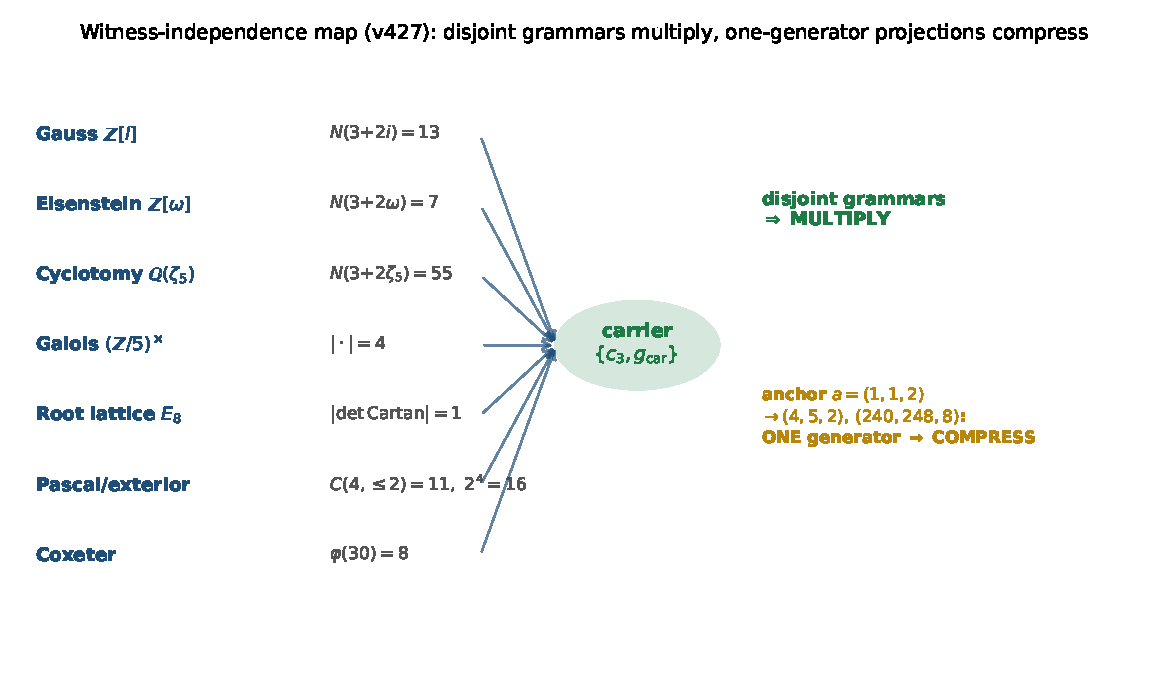
\includegraphics[width=0.92\linewidth]{figures/safeguard_witness_map}
\caption{The corrected over-determination map (\veri{v428\_overdet\_reclass.py}): the seven arithmetic
readouts are facets of \emph{one} $(2,3,5)/E_8$ object (a \emph{compression} gain, like the anchor), so they
do not multiply; what genuinely multiplies is the input forced four independent ways (the ``$8$'') plus the
foreign witness $\alpha^{-1}\!\approx\!137$.}\label{fig:witness}
\end{figure}

\section{Layer 4 --- the firewall and the No-Unit theorem}
Two safeguards keep the boundary between the closed core and external physics sharp.
\begin{itemize}
\item \textbf{The firewall.} The four frontier transfers --- $F_{\mathrm{pole}}$ (Koide),
$F_{\mathrm{Boltzmann}}$ ($\eta_B$), $F_{\mathrm{relic}}$ (axion), $F_{\mathrm{QCD}}$ ($m_p/m_e$) --- are
\emph{typed interfaces}, a discrete compiler kernel composed with an external continuous solver. A guard
(\veri{v187\_ftransfer\_laws.py}) reads the ledger and \emph{enforces} that none is ever typed as a
primitive \mE\ compiler prediction; the functor contract is \veri{v213\_ftransfer\_functor.py} and a prose
sentinel (\veri{v188\_frontier\_wording\_guard.py}) guards the wording. Exact algebraic sub-parts may be
\mE\ (the Koide $53/54$ factor, $b_3=-7$); the physical observable never is. The recent single-flow reduction (\veri{v425\_dyn\_transfer\_universal.py})
makes the \emph{dynamics} of all four the one native seam recovery semigroup, leaving only named anchors
external --- a sharpening that respects, not relaxes, the firewall.
\item \textbf{The No-Unit theorem} (\veri{v153\_no\_unit\_theorem.py}). Because $\cthree$ and $\gcar$ are
mass-dimension $0$, no dimensionless compiler can output an absolute scale; $v_{\mathrm{geo}}$ is therefore
\emph{forbidden by theorem}, not a missing prediction. The residual-certification audit
(\veri{v384\_residual\_certification.py}) makes the shape explicit: every open item is an external math
proof, theorem-forbidden (the unit), or external physics --- \emph{zero} open internal mechanisms.
\end{itemize}

\section{Layer 5 --- frozen predictions, the null model, and the $\alpha$ uniqueness scan}
Predictions are frozen before confrontation, and a match is scored against \emph{chance}, not admired in
isolation.
\begin{keybox}[The look-elsewhere null model, made explicit (\veri{v100\_numerology\_null\_mc.py})]
The frozen registry (\veri{v84\_frozen\_registry.py}, \texttt{REG.FREEZE.01}) fixes every dimensionless
prediction at $25$ digits, re-derived from the two axioms each run (a formula$\leftrightarrow$value lock).
The null model then runs an \emph{exact census} of the full declared formula grammar over the $13$ scored
observables with conservative data windows: the joint formula-fishing probability is $\prod_i p_i=10^{-25.8}$,
and $2{\times}200{,}000$ Monte-Carlo pseudo-theories reach \emph{at most} $5/13$ hits against TFPT's $13/13$
(Fig.~\ref{fig:nullmc}). Power controls confirm the test bites: $\phiz\pm10\%$ collapses TFPT's own
scorecard to $6/13$, and a data shuffle averages $1.2/13$.
\end{keybox}
\begin{figure}[ht]\centering
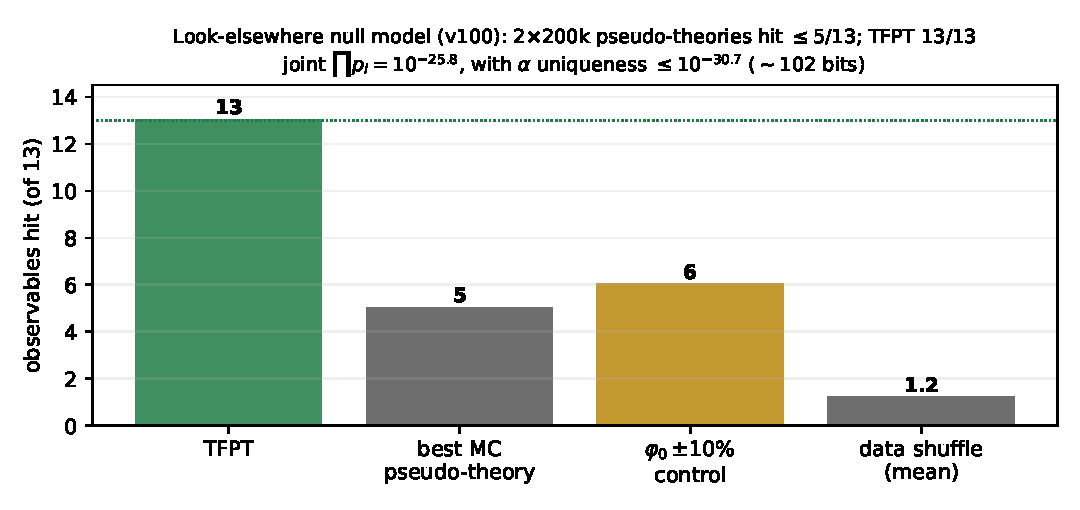
\includegraphics[width=0.72\linewidth]{figures/safeguard_null_model}
\caption{The look-elsewhere null model (\veri{v100\_numerology\_null\_mc.py}): Monte-Carlo pseudo-theories
hit at most $5/13$ where TFPT hits $13/13$; the power controls ($\phiz\pm10\%$, data shuffle) confirm the
test is non-vacuous.}\label{fig:nullmc}
\end{figure}
\par\smallskip\noindent\textbf{Is the $\alpha$ path unique?} The sharpest single result is the
fine-structure fixed point. All $94{,}500$ variants of the boundary $U(1)$ Ward formula $F_{U(1)}$ in the
declared grammar are root-solved; \emph{exactly one} --- the budget $M{=}41$ at $N{=}8$ ($\cthree=1/8\pi$)
--- lands in the $4{\times}10^{-8}$ CODATA window (Fig.~\ref{fig:alpha}). Folding this into the census gives
a total $\le10^{-30.7}$ ($\sim$102 bits), \emph{conditional on the declared grammar} --- a null-model
rejection, never a claim of certainty.
\begin{figure}[ht]\centering
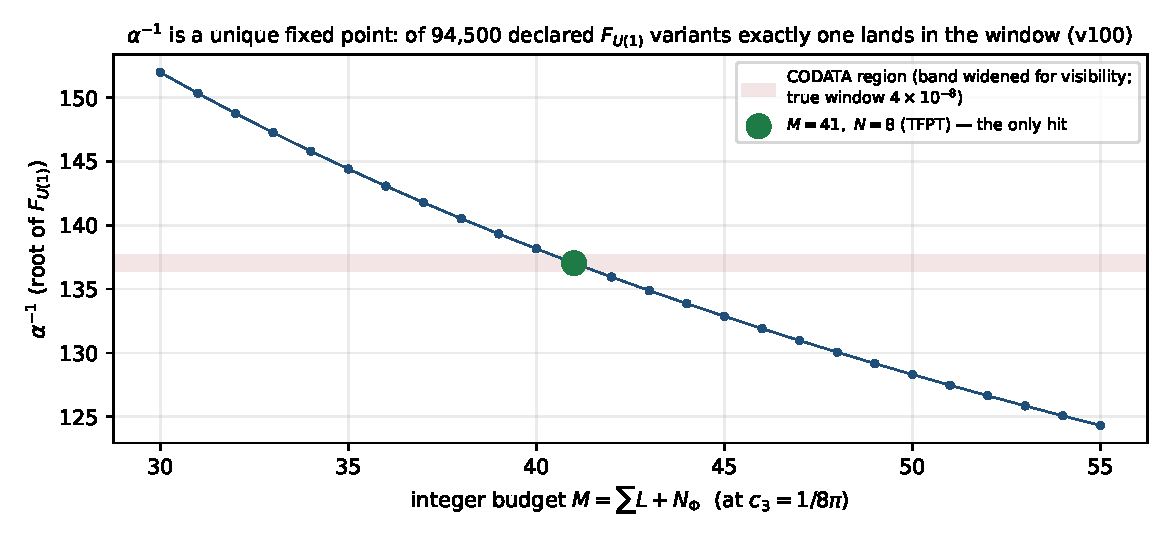
\includegraphics[width=0.80\linewidth]{figures/safeguard_alpha_uniqueness}
\caption{$\alpha^{-1}$ as a unique fixed point: scanning the integer budget $M$ at $\cthree=1/8\pi$, only
$M{=}41$ lands in the CODATA window; the full census over all $94{,}500$ $F_{U(1)}$ variants finds exactly
one hit.}\label{fig:alpha}
\end{figure}
\par\smallskip\noindent\textbf{No moving goalposts; the worst case is shown.} A live data scorecard records
the JUNO/NuFIT/ACT/BK18 compatibility (\veri{v375\_observatory\_registry.py}). A data watchdog types each row
as PASS, WATCH, TENSION or KILL (\veri{v307\_data\_watchdog.py}), and a kill-test board keeps the falsifiers
tied to the frozen rows (\veri{v321\_killtest\_board.py}). The discipline is applied to its own weakest
point: the reactor angle $\sin^2\theta_{13}=\phiz\,e^{-5/6}$ is \emph{pre-registered} at $+2.0\sigma$ tension
(\texttt{FLAV.TH13.PRESSURE.01}) with its own kill criterion --- the opposite of hiding the worst case.

\section{Layer 6 --- two independent reproduction paths}
A single implementation can share a single bug; TFPT therefore re-derives the exact core twice more,
independently.
\begin{itemize}
\item \textbf{An independent Wolfram engine} (\texttt{GATE.WOLFRAM.01}/\texttt{GATE.WOLFRAM.02}):
$116/116$ base checks plus a $327/327$ extension mirror every exact algebraic / identity / lattice result
in a different computer-algebra system, ending \texttt{ALL WOLFRAM CHECKS PASSED}. (Numerical ODE/PDE
results are Python-only by design and flagged as such.)
\item \textbf{A Lean~4 kernel proof}: the load-bearing algebra is machine-formalised with no \texttt{sorry}
--- the carrier hypercharge as the exact anomaly-free root of $6Y^2{-}Y{-}1=0$, the Pascal carrier
ladder $2^4=\binom50{+}\binom51{+}\binom52$ (\texttt{FORM.LADDER.01}), the integer rigidity of the carrier,
the seam-equivalence chain (\texttt{FORM.SEAMEQUIV.01}) and its collar/MMST face
(\texttt{FORM.SEAM.MMST.01}) --- so the kernel, not the prose, certifies the core.
\end{itemize}

\section{Layer 7 --- the red team}
The adversarial audit (companion \texttt{tfpt\_5\_redteam}) does not defend; it \emph{attacks}. It declares
six targets --- A (the seam$\,=\,(E_8)_1$ identification), B (the carrier truncation $\gcar{=}5$), C (the
$k{=}c_3/2$ area law), D (the ratios$\,\to v_{\mathrm{geo}}$ reduction), E (whether one scale carries the
theory), F (the perturbative 4D-QFT round) --- states what survives each, and reduces every survivor to a
named residual. The model
example is its own honesty about holomorphy: $c=8$ alone does \emph{not} select $(E_8)_1$ because
$(D_8)_1=SO(16)_1$ shares $c=8$; the load-bearing extra is holomorphy ($|\!\det K|=1$). Publishing the
sharpest attack on oneself is the strongest anti-numerology signal a programme can give.

\section{What would still falsify TFPT}
The safeguards are only credible with explicit kill tests (companion ``How to kill TFPT''). Among the
frozen ones: a fourth chiral generation (breaks $\Nfam=3$); a genuinely free fundamental constant that is
not an $E_8$-closure fixed point; a seam denominator $\neq 8$; $\ainv$ away from the fixed-point root; a
stable $\sin^2\theta_{13}$ far from $0.0231$ at $>3\sigma$; cosmic birefringence converging away from
$\beta\approx0.2424^\circ$; a tensor-to-scalar $r\gtrsim0.01$ (which kills the $R^2$ branch). The honest
residual above all kill tests is exactly three named interfaces --- the seam continuum theorem
($\texttt{SEAM.EQUIV.01}$, now reduced to a cited commuting-projector result,
\veri{v424\_seam\_lto\_rp\_reduction.py}/\veri{v426\_seam\_lto\_rp\_kms.py}), the metrology unit
$v_{\mathrm{geo}}$ (theorem-forbidden), and the typed $F_{\mathrm{transfer}}$ interfaces (firewalled).

\section{Summary --- the layered defense}
\begin{center}\small
\begin{tabularx}{\linewidth}{@{}lYl@{}}
\toprule
\textbf{Layer} & \textbf{What it defends against} & \textbf{Artefact} \\
\midrule
Status calculus & a \mC\ claim read as \mE & ledger $+$ \texttt{audit\_sync.py} \\
No free pattern $+$ reverse audit & cherry-picking, decorative identities & \vref{v305}/\vref{v100}/\texttt{E8.REVERSE.AUDIT.01} \\
Over-determination map & rhetorical ``everything multiplies'' (incl.\ \emph{our own} miscount) & \vref{v427}/\vref{v428} \\
Firewall $+$ No-Unit & external physics sold as compiler output; a faked scale & \vref{v187}/\vref{v213}/\vref{v153}/\vref{v384} \\
Frozen registry $+$ null model & moving goalposts; chance hits & \vref{v84}/\vref{v100}/\vref{v375} \\
Two independent paths & a shared implementation bug & Wolfram $+$ Lean \\
Red team & self-serving framing & \texttt{tfpt\_5\_redteam} \\
\bottomrule
\end{tabularx}
\end{center}
\noindent The claim defended here is deliberately narrow: \emph{coincidence is an expensive explanation of
the discrete core, and exact compiler closure is never silently upgraded to physical closure}. That is the
whole job of this companion.

\end{document}
